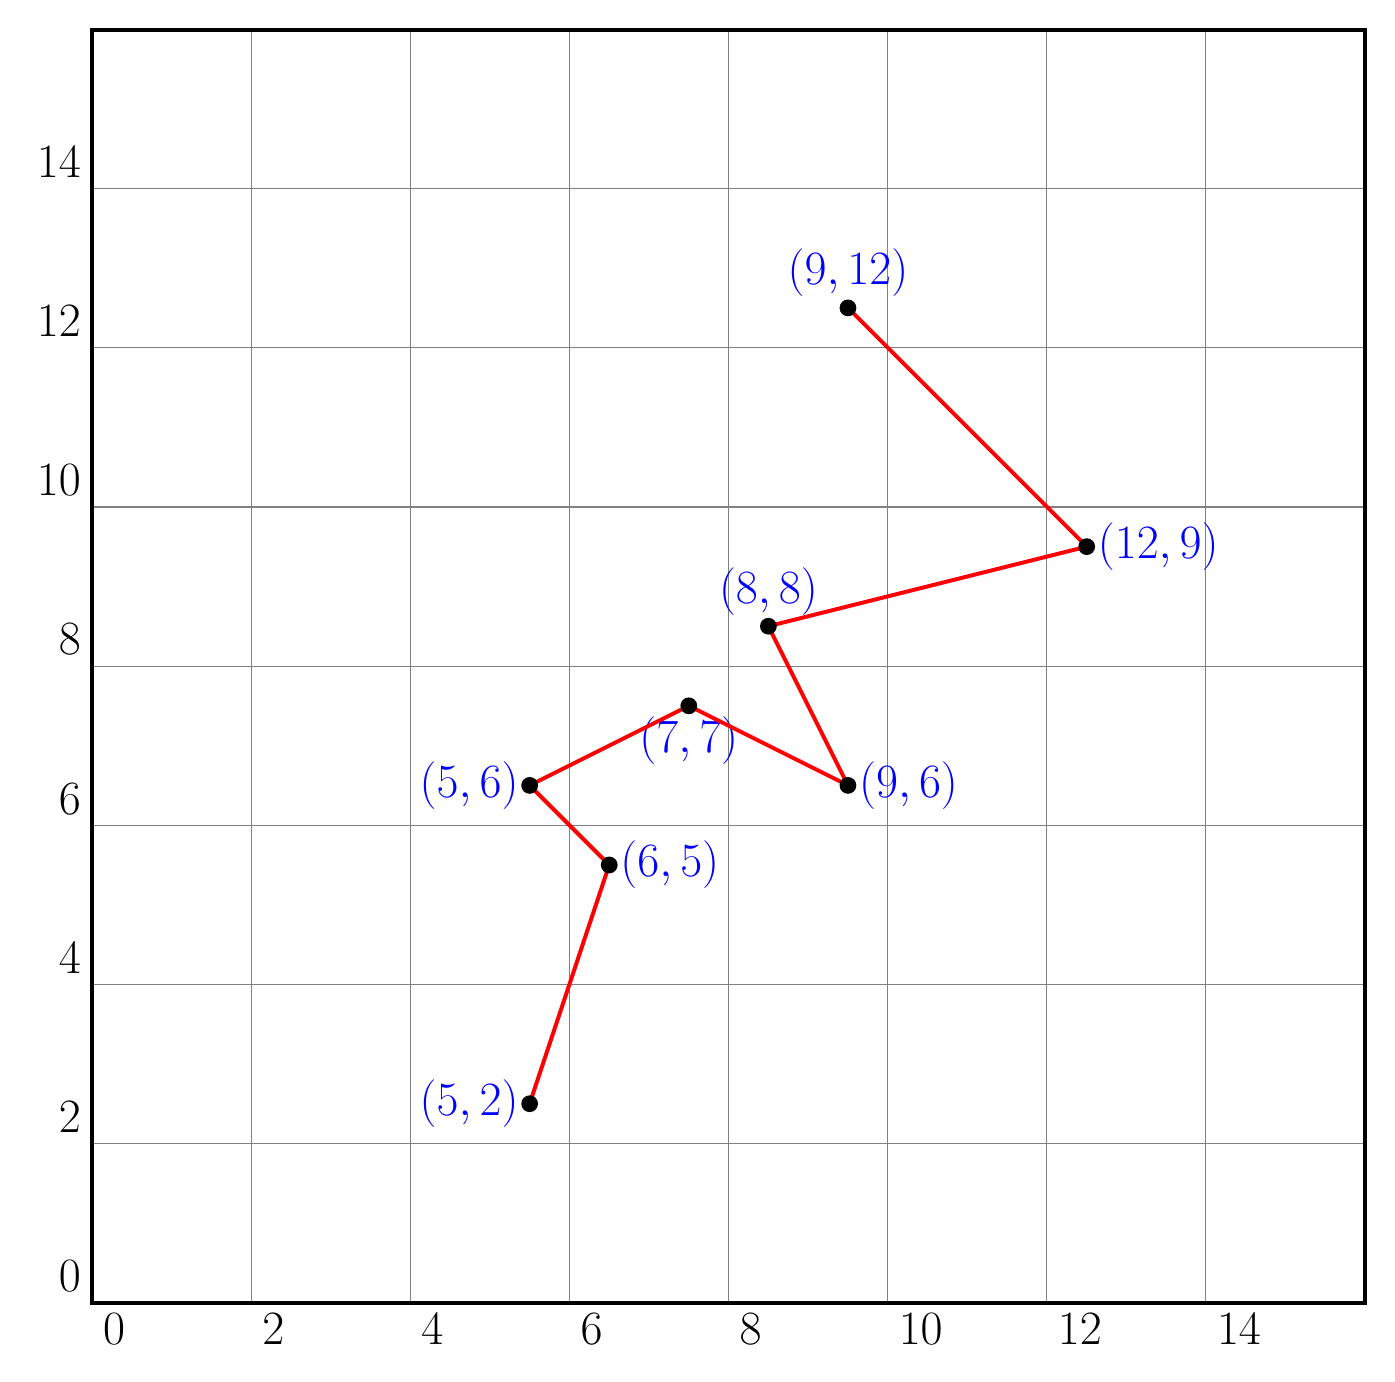
\begin{tikzpicture}[scale=\textwidth/12cm, line width=.5mm,
    morton/.style={every path/.style={draw=red}}]
    \def\A{\LARGE{\textcolor{blue}{$(5, 2)$}}}
    \def\B{\LARGE{\textcolor{blue}{$(6, 5)$}}}
    \def\C{\LARGE{\textcolor{blue}{$(5, 6)$}}}
    \def\D{\LARGE{\textcolor{blue}{$(7, 7)$}}}
    \def\E{\LARGE{\textcolor{blue}{$(9, 6)$}}}
    \def\F{\LARGE{\textcolor{blue}{$(8, 8)$}}}
    \def\G{\LARGE{\textcolor{blue}{$(12, 9)$}}}
    \def\H{\LARGE{\textcolor{blue}{$(9, 12)$}}}

    \draw[step=2cm,gray,thin] (0, 0) grid (16, 16);
    \draw (0, 0) rectangle (16, 16);

    \coordinate [label=left:\A] (A) at (5.5, 2.5);
    \coordinate [label=right:\B] (B) at (6.5, 5.5);
    \coordinate [label=left:\C] (C) at (5.5, 6.5);
    \coordinate [label=below:\D] (D) at (7.5, 7.5);
    \coordinate [label=right:\E] (E) at (9.5, 6.5);
    \coordinate [label=above:\F] (F) at (8.5, 8.5);
    \coordinate [label=right:\G] (G) at (12.5, 9.5);
    \coordinate [label=above:\H] (H) at (9.5, 12.5);

    \foreach \p in {0,2,...,14}{%
        \draw (0,\p) node[anchor=south east] {\LARGE{$\p$}};
        \draw (\p,0) node[anchor=north west] {\LARGE{$\p$}};
    }

    \begin{scope}[morton]
    \draw (A) -- (B);
    \draw (B) -- (C);
    \draw (C) -- (D);
    \draw (D) -- (E);
    \draw (E) -- (F);
    \draw (F) -- (G);
    \draw (G) -- (H);
    \end{scope}

    \foreach \point in {A, B, C, D, E, F, G, H}
        \fill [black] (\point) circle (3pt);
\end{tikzpicture}

% vim: set ff=unix tw=79 sw=4 ts=4 et ic ai :
